\chapter*{Appendix}
\centering
\def\pieData{52.2/Male, 47.8/Female}

% 2) Colors (pgf list) and count
\def\pieColors{{"SkyBlue", "Thistle"}}
\def\colorCount{7}

% 3) Pie geometry
\def\startAngle{90}       % where slice #1 begins (90° = top)
\def\pieRadius{3cm}       % radius of the pie

% 4) Legend styling & placement
\def\legendDist{1cm}      % horizontal gap between pie and legend
\def\lineSep{0.8cm}       % vertical separation between legend items
\def\labelFont{\small}    % legend font size
% ───────────────────────────────────

\begin{figure}[h]
  \centering
  \begin{tikzpicture}[nodes={font=\labelFont}]
    % ─── Draw the pie ───
    \newcount\sliceIdx \sliceIdx=-1
    \def\angle{\startAngle}
    \foreach \percent/\name in \pieData {%
      \global\advance\sliceIdx by 1
      \ifnum\sliceIdx>\numexpr\colorCount-1\relax
        \global\sliceIdx=0
      \fi
      \pgfmathparse{\pieColors[\the\sliceIdx]}\edef\sliceColor{\pgfmathresult}
      \draw[fill=\sliceColor!50,draw=\sliceColor]
        (0,0) -- (\angle:\pieRadius)
        arc(\angle:\angle-\percent*3.6:\pieRadius) -- cycle;
      \pgfmathparse{\angle-\percent*3.6}\xdef\angle{\pgfmathresult}
    }

    % ─── Compute legend anchor ───
    % This puts the top legend entry at (pieRadius + legendDist, +pieRadius)
    \coordinate (legendBase) at 
      ({\pieRadius+\legendDist}, {\pieRadius});

    % ─── Draw the legend ───
    \foreach [count=\i from 0] \percent/\name in \pieData {%
      \pgfmathparse{\pieColors[\i]}\edef\legendColor{\pgfmathresult}
      % colored box
      \fill[\legendColor!50]
        ($(legendBase)+(0,-\i*\lineSep)$) rectangle ++(6pt,-6pt);
      \draw
        ($(legendBase)+(0,-\i*\lineSep)$) rectangle ++(6pt,-6pt);
      % label text
      \node[anchor=west]
        at 
        ($ (legendBase)+(0,-\i*\lineSep) + (8pt,-3pt) $)
        {\name\ [\percent\%]};
    }
  \end{tikzpicture}
  \caption{Pie Chart of Gender}
\end{figure}

\begin{figure}[h]
    \centering
    % start at 90°
    \def\angle{90}%
    \def\radius{2}%
    \def\cyclelist{{"red","magenta","orange","green","cyan","violet","yellow"}}%
  
    \newcount\cyclecount \cyclecount=-1
    \newcount\ind        \ind=-1
    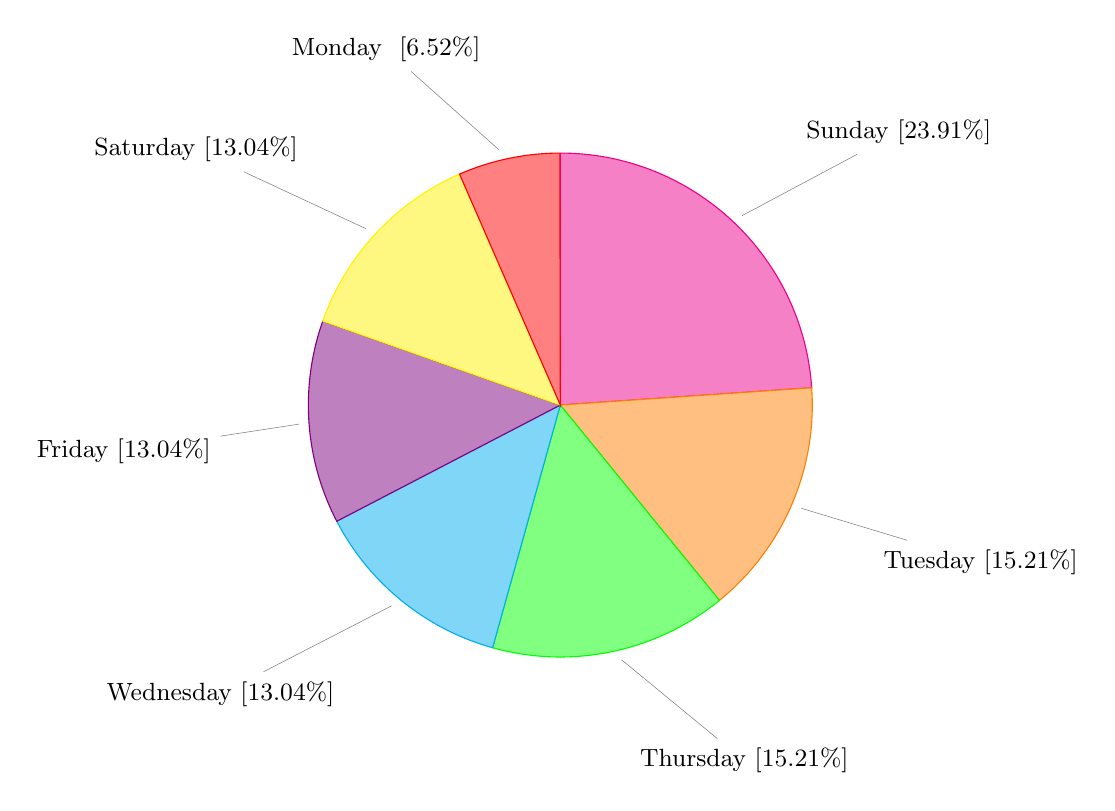
\begin{tikzpicture}[nodes={font=\small}, scale=1.6]
      % sorted descending: Sunday first (23.91%), …, Monday last (6.52%)
      \foreach \percent/\name in {
        23.91/Sunday,
        15.21/Tuesday,
        15.21/Thursday,
        13.04/Wednesday,
        13.04/Friday,
        13.04/Saturday,
        6.52/Monday
      }{%
        % cycle through colors
        \global\advance\cyclecount by 1
        \global\advance\ind        by 1
        \ifnum\cyclecount>6
          \global\cyclecount=0
          \global\ind       =0
        \fi
        \pgfmathparse{\cyclelist[\the\ind]}%
        \edef\color{\pgfmathresult}%
  
        % draw slice CLOCKWISE by subtracting degrees
        \draw[fill=\color!50, draw=\color]
          (0,0) -- (\angle:\radius)
          arc (\angle:\angle-\percent*3.6:\radius) -- cycle;
  
        % place the pin at the slice‐midpoint (angle minus half the sweep)
        \node[pin={[pin distance=1cm]\angle-0.5*\percent*3.6:{\name\ [\percent\%]}}]
          at (\angle-0.5*\percent*3.6:\radius) {};
  
        % advance the start angle
        \pgfmathparse{\angle-\percent*3.6}%
        \xdef\angle{\pgfmathresult}%
      }
    \end{tikzpicture}
  
    \caption{Pie chart of days with the highest screen time (sorted largest→smallest, clockwise)}
\end{figure}

\begin{center}
    % \begin{figure}[ht]
    %     \begin{tikzpicture}
    %         \pie[text=legend, rotate=90]{2.2/Information and Reading, 4.3/Education, 34.8/Social, 58.7/Entertainment}
    %     \end{tikzpicture}
    %     \caption{Pie chart of the most use application type}
    % \end{figure}
    % ──────────────── User settings ─────────────────
    % 1) Your data: comma-separated list of “percent/label”
    \def\pieData{2.2/Information and Reading, 4.3/Education, 34.8/Social, 58.7/Entertainment}

    % 2) Color cycle (must be a pgf list) and its length
    \def\pieColors{{"orange","blue","gray","red"}}
    \def\colorCount{7}

    % 3) Chart geometry & label style
    \def\startAngle{90}       % where slice #1 begins (90° = top)
    \def\pieRadius{3cm}       % radius of pie
    \def\pinDistance{1.2cm}    % how long the “pin” sticks out
    % \def\labelFont{\scriptsize} % font size for labels
    % ─────────────────────────────────────────────────

    \begin{figure}[h]
    \centering
    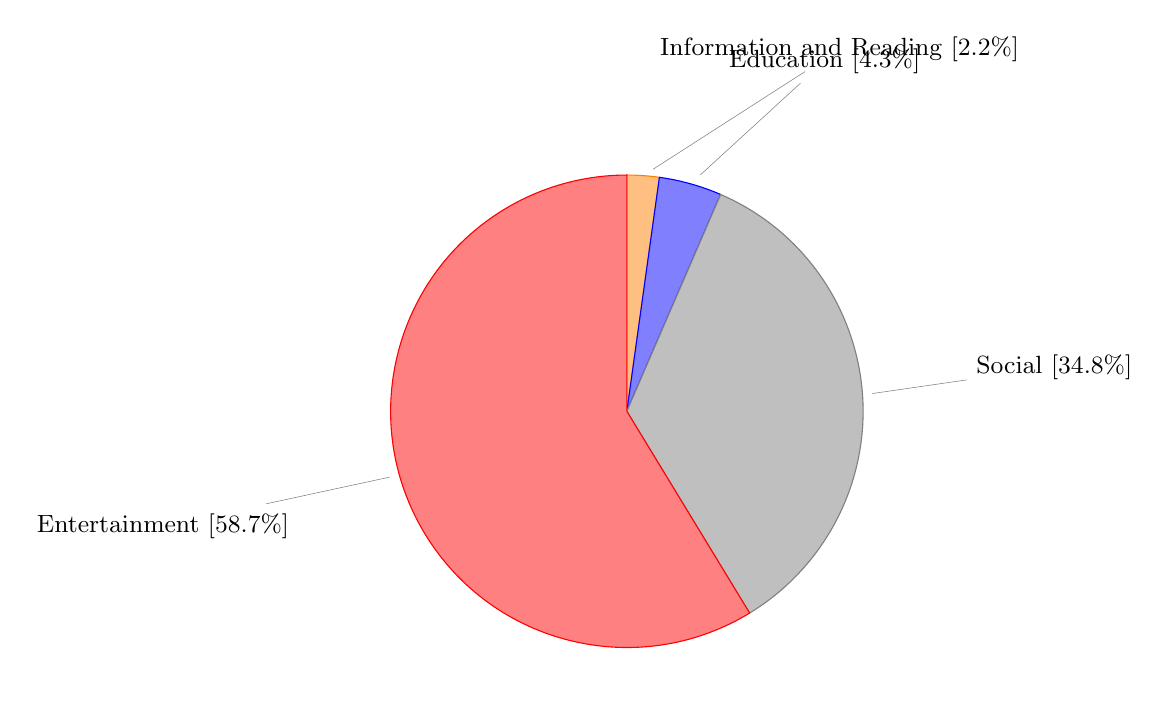
\begin{tikzpicture}[
        nodes={font=\labelFont},
        every pin/.append style={pin distance=\pinDistance}
    ]
    % internal counters
    \newcount\sliceIndex \sliceIndex=-1
    \def\angle{\startAngle}

    \foreach \percent/\name in \pieData {%
        % cycle through colors
        \global\advance\sliceIndex by 1
        \ifnum\sliceIndex>\numexpr\colorCount-1\relax
        \global\sliceIndex=0
        \fi
        \pgfmathparse{\pieColors[\the\sliceIndex]}%
        \edef\sliceColor{\pgfmathresult}%

        % draw one slice (clockwise)
        \draw[fill=\sliceColor!50,draw=\sliceColor]
        (0,0) -- (\angle:\pieRadius)
        arc(\angle:\angle-\percent*3.6:\pieRadius) -- cycle;

        % compute midpoint angle for label
        \pgfmathparse{\angle - 0.5*(\percent*3.6)}%
        \edef\midAngle{\pgfmathresult}%

        % place pin label
        \node[pin={[pin distance=\pinDistance]\midAngle:{\name\ [\percent\%]}}]
        at (\midAngle:\pieRadius) {};

        % advance start angle
        \pgfmathparse{\angle - \percent*3.6}%
        \xdef\angle{\pgfmathresult}%
    }
    \end{tikzpicture}
    \caption{Pie chart (largest→smallest, clockwise from 90°).}
    \end{figure}

    \begin{figure}[ht]
        \begin{tikzpicture}
            \pie[text=legend, rotate=90]{2.2/Friday, 8.7/Tuesday, 10.9/Sunday, 10.9/Wednesday, 19.6/Saturday, 19.6/Thursday, 28.3/Monday}
        \end{tikzpicture}
        \caption{Pie chart of day with the lowest screen time}
    \end{figure}

    \begin{figure}[ht]
        \begin{tikzpicture}
            \pie[text=legend, rotate=90]{2.17/Cataract, 2.17/Color blindness, 2.17/Pinguecula, 23.9/Astigmatism, 69.6/None}
        \end{tikzpicture}
        \caption{Pie chart of other eyesight problem}
    \end{figure}
\end{center}\\
\begin{table}[ht]
    \caption{Left eye}
    \begin{adjustbox}{width = \textwidth, center}
        \begin{tabular}{|cc|r|r|r|r|r|r|r|r|r|r|r|r|r|r|r|}
        \hline
        \multicolumn{2}{|c|}{}                                                          & \multicolumn{1}{c|}{\cellcolor[HTML]{F4CCCC}2} & \multicolumn{1}{c|}{\cellcolor[HTML]{F4CCCC}3} & \multicolumn{1}{c|}{\cellcolor[HTML]{F4CCCC}4} & \multicolumn{1}{c|}{\cellcolor[HTML]{F4CCCC}5} & \multicolumn{1}{c|}{\cellcolor[HTML]{F4CCCC}6} & \multicolumn{1}{c|}{\cellcolor[HTML]{F4CCCC}7} & \multicolumn{1}{c|}{\cellcolor[HTML]{F4CCCC}8} & \multicolumn{1}{c|}{\cellcolor[HTML]{F4CCCC}9}  & \multicolumn{1}{c|}{\cellcolor[HTML]{F4CCCC}10} & \multicolumn{1}{c|}{\cellcolor[HTML]{F4CCCC}11} & \multicolumn{1}{c|}{\cellcolor[HTML]{F4CCCC}12} & \multicolumn{1}{c|}{\cellcolor[HTML]{F4CCCC}13} & \multicolumn{1}{c|}{\cellcolor[HTML]{D9D2E9}}                                   & \multicolumn{1}{c|}{\cellcolor[HTML]{D9D2E9}}                           & \multicolumn{1}{c|}{\cellcolor[HTML]{D9D2E9}}                                                    \\
        \multicolumn{2}{|c|}{\multirow{-2}{*}{\backslashbox{$y$}{$x$}}}                 & \multicolumn{1}{c|}{\cellcolor[HTML]{FFEBEA}3} & \multicolumn{1}{c|}{\cellcolor[HTML]{FFEBEA}4} & \multicolumn{1}{c|}{\cellcolor[HTML]{FFEBEA}5} & \multicolumn{1}{c|}{\cellcolor[HTML]{FFEBEA}6} & \multicolumn{1}{c|}{\cellcolor[HTML]{FFEBEA}7} & \multicolumn{1}{c|}{\cellcolor[HTML]{FFEBEA}8} & \multicolumn{1}{c|}{\cellcolor[HTML]{FFEBEA}9} & \multicolumn{1}{c|}{\cellcolor[HTML]{FFEBEA}10} & \multicolumn{1}{c|}{\cellcolor[HTML]{FFEBEA}11} & \multicolumn{1}{c|}{\cellcolor[HTML]{FFEBEA}12} & \multicolumn{1}{c|}{\cellcolor[HTML]{FFEBEA}13} & \multicolumn{1}{c|}{\cellcolor[HTML]{FFEBEA}14} & \multicolumn{1}{c|}{\multirow{-2}{*}{\cellcolor[HTML]{D9D2E9}$\widehat{P}(Y)$}} & \multicolumn{1}{c|}{\multirow{-2}{*}{\cellcolor[HTML]{D9D2E9}midpoint}} & \multicolumn{1}{c|}{\multirow{-2}{*}{\cellcolor[HTML]{D9D2E9}$\mathrm{mid}\cdot\widehat{P}(Y)$}} \\ \hline
        \rowcolor[HTML]{FFFFFF} 
        \cellcolor[HTML]{D0E0E3}-850           & \cellcolor[HTML]{EBF1FC}-750           & 0                                              & 0                                              & 0                                              & 0                                              & 0                                              & 0                                              & \cellcolor[HTML]{C7E9D8}0.0227                 & 0                                               & 0                                               & 0                                               & 0                                               & 0                                               & \cellcolor[HTML]{D9D2E9}0.0227                                                  & \cellcolor[HTML]{D9D2E9}-800                                            & \cellcolor[HTML]{D9D2E9}-18.18181818                                                             \\ \hline
        \rowcolor[HTML]{FFFFFF} 
        \cellcolor[HTML]{D0E0E3}-750           & \cellcolor[HTML]{EBF1FC}-650           & 0                                              & 0                                              & 0                                              & 0                                              & 0                                              & 0                                              & 0                                              & 0                                               & 0                                               & 0                                               & 0                                               & 0                                               & \cellcolor[HTML]{D9D2E9}0                                                       & \cellcolor[HTML]{D9D2E9}-700                                            & \cellcolor[HTML]{D9D2E9}0                                                                        \\ \hline
        \rowcolor[HTML]{FFFFFF} 
        \cellcolor[HTML]{D0E0E3}-650           & \cellcolor[HTML]{EBF1FC}-550           & 0                                              & 0                                              & 0                                              & 0                                              & \cellcolor[HTML]{C7E9D8}0.0227                 & \cellcolor[HTML]{C7E9D8}0.0227                 & 0                                              & 0                                               & 0                                               & 0                                               & 0                                               & 0                                               & \cellcolor[HTML]{D9D2E9}0.0455                                                  & \cellcolor[HTML]{D9D2E9}-600                                            & \cellcolor[HTML]{D9D2E9}-27.27272727                                                             \\ \hline
        \rowcolor[HTML]{FFFFFF} 
        \cellcolor[HTML]{D0E0E3}-550           & \cellcolor[HTML]{EBF1FC}-450           & 0                                              & \cellcolor[HTML]{C7E9D8}0.0227                 & 0                                              & 0                                              & 0                                              & 0                                              & 0                                              & 0                                               & 0                                               & 0                                               & 0                                               & 0                                               & \cellcolor[HTML]{D9D2E9}0.0227                                                  & \cellcolor[HTML]{D9D2E9}-500                                            & \cellcolor[HTML]{D9D2E9}-11.36363636                                                             \\ \hline
        \rowcolor[HTML]{FFFFFF} 
        \cellcolor[HTML]{D0E0E3}-450           & \cellcolor[HTML]{EBF1FC}-350           & 0                                              & 0                                              & 0                                              & \cellcolor[HTML]{8FD2B1}0.0455                 & 0                                              & 0                                              & \cellcolor[HTML]{C7E9D8}0.0227                 & 0                                               & \cellcolor[HTML]{C7E9D8}0.0227                  & 0                                               & 0                                               & 0                                               & \cellcolor[HTML]{D9D2E9}0.0909                                                  & \cellcolor[HTML]{D9D2E9}-400                                            & \cellcolor[HTML]{D9D2E9}-36.36363636                                                             \\ \hline
        \cellcolor[HTML]{D0E0E3}-350           & \cellcolor[HTML]{EBF1FC}-250           & \cellcolor[HTML]{FFFFFF}0                      & \cellcolor[HTML]{C7E9D8}0.0227                 & \cellcolor[HTML]{C7E9D8}0.0227                 & \cellcolor[HTML]{FFFFFF}0                      & \cellcolor[HTML]{FFFFFF}0                      & \cellcolor[HTML]{C7E9D8}0.0227                 & \cellcolor[HTML]{FFFFFF}0                      & \cellcolor[HTML]{C7E9D8}0.0227                  & \cellcolor[HTML]{FFFFFF}0                       & \cellcolor[HTML]{FFFFFF}0                       & \cellcolor[HTML]{FFFFFF}0                       & \cellcolor[HTML]{FFFFFF}0                       & \cellcolor[HTML]{D9D2E9}0.0909                                                  & \cellcolor[HTML]{D9D2E9}-300                                            & \cellcolor[HTML]{D9D2E9}-27.27272727                                                             \\ \hline
        \cellcolor[HTML]{D0E0E3}-250           & \cellcolor[HTML]{EBF1FC}-150           & \cellcolor[HTML]{C7E9D8}0.0227                 & \cellcolor[HTML]{FFFFFF}0                      & \cellcolor[HTML]{FFFFFF}0                      & \cellcolor[HTML]{C7E9D8}0.0227                 & \cellcolor[HTML]{C7E9D8}0.0227                 & \cellcolor[HTML]{C7E9D8}0.0227                 & \cellcolor[HTML]{FFFFFF}0                      & \cellcolor[HTML]{FFFFFF}0                       & \cellcolor[HTML]{FFFFFF}0                       & \cellcolor[HTML]{FFFFFF}0                       & \cellcolor[HTML]{FFFFFF}0                       & \cellcolor[HTML]{FFFFFF}0                       & \cellcolor[HTML]{D9D2E9}0.0909                                                  & \cellcolor[HTML]{D9D2E9}-200                                            & \cellcolor[HTML]{D9D2E9}-18.18181818                                                             \\ \hline
        \cellcolor[HTML]{D0E0E3}-150           & \cellcolor[HTML]{EBF1FC}-50            & \cellcolor[HTML]{FFFFFF}0                      & \cellcolor[HTML]{C7E9D8}0.0227                 & \cellcolor[HTML]{C7E9D8}0.0227                 & \cellcolor[HTML]{C7E9D8}0.0227                 & \cellcolor[HTML]{FFFFFF}0                      & \cellcolor[HTML]{C7E9D8}0.0227                 & \cellcolor[HTML]{FFFFFF}0                      & \cellcolor[HTML]{FFFFFF}0                       & \cellcolor[HTML]{FFFFFF}0                       & \cellcolor[HTML]{FFFFFF}0                       & \cellcolor[HTML]{FFFFFF}0                       & \cellcolor[HTML]{C7E9D8}0.0227                  & \cellcolor[HTML]{D9D2E9}0.1136                                                  & \cellcolor[HTML]{D9D2E9}-100                                            & \cellcolor[HTML]{D9D2E9}-11.36363636                                                             \\ \hline
        \cellcolor[HTML]{D0E0E3}-50            & \cellcolor[HTML]{EBF1FC}50             & \cellcolor[HTML]{8FD2B1}0.0455                 & \cellcolor[HTML]{57BB8A}0.0682                 & \cellcolor[HTML]{8FD2B1}0.0455                 & \cellcolor[HTML]{57BB8A}0.0682                 & \cellcolor[HTML]{8FD2B1}0.0455                 & \cellcolor[HTML]{8FD2B1}0.0455                 & \cellcolor[HTML]{57BB8A}0.0682                 & \cellcolor[HTML]{57BB8A}0.0682                  & \cellcolor[HTML]{FFFFFF}0                       & \cellcolor[HTML]{FFFFFF}0                       & \cellcolor[HTML]{FFFFFF}0                       & \cellcolor[HTML]{FFFFFF}0                       & \cellcolor[HTML]{D9D2E9}0.4545                                                  & \cellcolor[HTML]{D9D2E9}0                                               & \cellcolor[HTML]{D9D2E9}0                                                                        \\ \hline
        \rowcolor[HTML]{FFFFFF} 
        \cellcolor[HTML]{D0E0E3}50             & \cellcolor[HTML]{EBF1FC}150            & 0                                              & 0                                              & 0                                              & 0                                              & 0                                              & 0                                              & 0                                              & 0                                               & 0                                               & 0                                               & 0                                               & 0                                               & \cellcolor[HTML]{D9D2E9}0                                                       & \cellcolor[HTML]{D9D2E9}100                                             & \cellcolor[HTML]{D9D2E9}0                                                                        \\ \hline
        \rowcolor[HTML]{FFFFFF} 
        \cellcolor[HTML]{D0E0E3}150            & \cellcolor[HTML]{EBF1FC}250            & 0                                              & 0                                              & 0                                              & \cellcolor[HTML]{C7E9D8}0.0227                 & 0                                              & 0                                              & \cellcolor[HTML]{C7E9D8}0.0227                 & 0                                               & 0                                               & 0                                               & 0                                               & 0                                               & \cellcolor[HTML]{D9D2E9}0.0455                                                  & \cellcolor[HTML]{D9D2E9}200                                             & \cellcolor[HTML]{D9D2E9}9.090909091                                                              \\ \hline
        \rowcolor[HTML]{FFFFFF} 
        \cellcolor[HTML]{D0E0E3}250            & \cellcolor[HTML]{EBF1FC}350            & 0                                              & 0                                              & \cellcolor[HTML]{C7E9D8}0.0227                 & 0                                              & 0                                              & 0                                              & 0                                              & 0                                               & 0                                               & 0                                               & 0                                               & 0                                               & \cellcolor[HTML]{D9D2E9}0.0227                                                  & \cellcolor[HTML]{D9D2E9}300                                             & \cellcolor[HTML]{D9D2E9}6.818181818                                                              \\ \hline
        \multicolumn{2}{|c|}{\cellcolor[HTML]{FFF2CC}$\widehat{P}(X)$}                  & \cellcolor[HTML]{FFF2CC}0.0682                 & \cellcolor[HTML]{FFF2CC}0.1364                 & \cellcolor[HTML]{FFF2CC}0.1136                 & \cellcolor[HTML]{FFF2CC}0.1818                 & \cellcolor[HTML]{FFF2CC}0.0909                 & \cellcolor[HTML]{FFF2CC}0.1364                 & \cellcolor[HTML]{FFF2CC}0.1364                 & \cellcolor[HTML]{FFF2CC}0.0909                  & \cellcolor[HTML]{FFF2CC}0.0227                  & \cellcolor[HTML]{FFF2CC}0                       & \cellcolor[HTML]{FFF2CC}0                       & \cellcolor[HTML]{FFF2CC}0.0227                  & \multicolumn{1}{l|}{}                                                           & \multicolumn{1}{l|}{}                                                   & \multicolumn{1}{l|}{}                                                                            \\ \hline
        \multicolumn{2}{|c|}{\cellcolor[HTML]{FFF2CC}midpoint}                          & \cellcolor[HTML]{FFF2CC}2.5                    & \cellcolor[HTML]{FFF2CC}3.5                    & \cellcolor[HTML]{FFF2CC}4.5                    & \cellcolor[HTML]{FFF2CC}5.5                    & \cellcolor[HTML]{FFF2CC}6.5                    & \cellcolor[HTML]{FFF2CC}7.5                    & \cellcolor[HTML]{FFF2CC}8.5                    & \cellcolor[HTML]{FFF2CC}9.5                     & \cellcolor[HTML]{FFF2CC}10.5                    & \cellcolor[HTML]{FFF2CC}11.5                    & \cellcolor[HTML]{FFF2CC}12.5                    & \cellcolor[HTML]{FFF2CC}13.5                    & \multicolumn{1}{l|}{}                                                           & \multicolumn{1}{l|}{\cellcolor[HTML]{F9CB9C}$\widehat{E}(X)$}           & \cellcolor[HTML]{F9CB9C}6.340909091                                                              \\ \hline
        \multicolumn{2}{|c|}{\cellcolor[HTML]{FFF2CC}$\mathrm{mid}\cdot\widehat{P}(X)$} & \cellcolor[HTML]{FFF2CC}0.1704545455           & \cellcolor[HTML]{FFF2CC}0.4772727273           & \cellcolor[HTML]{FFF2CC}0.5113636364           & \cellcolor[HTML]{FFF2CC}1                      & \cellcolor[HTML]{FFF2CC}0.5909090909           & \cellcolor[HTML]{FFF2CC}1.022727273            & \cellcolor[HTML]{FFF2CC}1.159090909            & \cellcolor[HTML]{FFF2CC}0.8636363636            & \cellcolor[HTML]{FFF2CC}0.2386363636            & \cellcolor[HTML]{FFF2CC}0                       & \cellcolor[HTML]{FFF2CC}0                       & \cellcolor[HTML]{FFF2CC}0.3068181818            & \multicolumn{1}{l|}{}                                                           & \multicolumn{1}{l|}{\cellcolor[HTML]{F9CB9C}$\widehat{E}(Y)$}           & \cellcolor[HTML]{F9CB9C}-134.0909091                                                             \\ \hline
        \end{tabular}
    \end{adjustbox}
\end{table}
\begin{table}
    \caption{Left eye correlation}
    \begin{adjustbox}{width = 0.4\textwidth, center}
        \begin{tabular}{|cll|c|}
            \hline
            \rowcolor[HTML]{FFE599} 
            \multicolumn{3}{|c|}{\cellcolor[HTML]{FFE599}Min X}                                   & Min Y      \\ \hline
            \multicolumn{3}{|c|}{2.2357}                                                          & -800       \\ \hline
            \rowcolor[HTML]{FFE599} 
            \multicolumn{3}{|c|}{\cellcolor[HTML]{FFE599}Max X}                                   & Max Y      \\ \hline
            \multicolumn{3}{|c|}{13.8500}                                                         & 250        \\ \hline
            \rowcolor[HTML]{FFE599} 
            \multicolumn{3}{|c|}{\cellcolor[HTML]{FFE599}$\overline{X}$}                                   & $\overline{Y}$      \\ \hline
            \multicolumn{3}{|c|}{6.3647}                                                          & -142.5000  \\ \hline
            \multicolumn{3}{|c|}{\cellcolor[HTML]{FFE599}$\sum(X-\overline{X})(Y-\overline{Y})}$                 & -3074.4167 \\ \hline
            \multicolumn{3}{|c|}{\cellcolor[HTML]{FFE599}$\widehat{\mathrm{cov}}_{X, Y}=\dfrac{\sum(X-\overline{X})(Y-\overline{Y})}{n-1}}$ & -69.8731   \\ \hline
            \multicolumn{3}{|c|}{\cellcolor[HTML]{FFE599}$s_X$}                                     & 2.4974     \\ \hline
            \multicolumn{3}{|c|}{\cellcolor[HTML]{FFE599}$s_Y$}                                     & 225.1834   \\ \hline
            \multicolumn{3}{|c|}{\cellcolor[HTML]{FFE599}$\rho_{X,Y}= \frac{\widehat{\mathrm{cov}}_{X, Y}}{s_X\cdot s_Y}}$        & -0.1242    \\ \hline
        \end{tabular}
    \end{adjustbox}
\end{table}\\
\begin{table}
    \begin{adjustbox}{width = \textwidth, center}
        \caption{Right eye}
        \begin{tabular}{|cc|
            >{\columncolor[HTML]{FFFFFF}}r |
            >{\columncolor[HTML]{FFFFFF}}r |
            >{\columncolor[HTML]{FFFFFF}}r |
            >{\columncolor[HTML]{FFFFFF}}r |
            >{\columncolor[HTML]{FFFFFF}}r |r|r|
            >{\columncolor[HTML]{FFFFFF}}r |
            >{\columncolor[HTML]{FFFFFF}}r |
            >{\columncolor[HTML]{FFFFFF}}r |
            >{\columncolor[HTML]{FFFFFF}}r |
            >{\columncolor[HTML]{FFFFFF}}r |r|r|r|}
            \hline
            \multicolumn{2}{|c|}{}                                                          & \multicolumn{1}{c|}{\cellcolor[HTML]{F4CCCC}2} & \multicolumn{1}{c|}{\cellcolor[HTML]{F4CCCC}3} & \multicolumn{1}{c|}{\cellcolor[HTML]{F4CCCC}4} & \multicolumn{1}{c|}{\cellcolor[HTML]{F4CCCC}5} & \multicolumn{1}{c|}{\cellcolor[HTML]{F4CCCC}6} & \multicolumn{1}{c|}{\cellcolor[HTML]{F4CCCC}7} & \multicolumn{1}{c|}{\cellcolor[HTML]{F4CCCC}8} & \multicolumn{1}{c|}{\cellcolor[HTML]{F4CCCC}9}  & \multicolumn{1}{c|}{\cellcolor[HTML]{F4CCCC}10} & \multicolumn{1}{c|}{\cellcolor[HTML]{F4CCCC}11} & \multicolumn{1}{c|}{\cellcolor[HTML]{F4CCCC}12} & \multicolumn{1}{c|}{\cellcolor[HTML]{F4CCCC}13} & \multicolumn{1}{c|}{\cellcolor[HTML]{D9D2E9}}                                   & \multicolumn{1}{c|}{\cellcolor[HTML]{D9D2E9}}                           & \multicolumn{1}{c|}{\cellcolor[HTML]{D9D2E9}}                                                    \\
            \multicolumn{2}{|c|}{\multirow{-2}{*}{\backslashbox{$y$}{$x$}}}                 & \multicolumn{1}{c|}{\cellcolor[HTML]{FFEBEA}3} & \multicolumn{1}{c|}{\cellcolor[HTML]{FFEBEA}4} & \multicolumn{1}{c|}{\cellcolor[HTML]{FFEBEA}5} & \multicolumn{1}{c|}{\cellcolor[HTML]{FFEBEA}6} & \multicolumn{1}{c|}{\cellcolor[HTML]{FFEBEA}7} & \multicolumn{1}{c|}{\cellcolor[HTML]{FFEBEA}8} & \multicolumn{1}{c|}{\cellcolor[HTML]{FFEBEA}9} & \multicolumn{1}{c|}{\cellcolor[HTML]{FFEBEA}10} & \multicolumn{1}{c|}{\cellcolor[HTML]{FFEBEA}11} & \multicolumn{1}{c|}{\cellcolor[HTML]{FFEBEA}12} & \multicolumn{1}{c|}{\cellcolor[HTML]{FFEBEA}13} & \multicolumn{1}{c|}{\cellcolor[HTML]{FFEBEA}14} & \multicolumn{1}{c|}{\multirow{-2}{*}{\cellcolor[HTML]{D9D2E9}$\widehat{P}(Y)$}} & \multicolumn{1}{c|}{\multirow{-2}{*}{\cellcolor[HTML]{D9D2E9}midpoint}} & \multicolumn{1}{c|}{\multirow{-2}{*}{\cellcolor[HTML]{D9D2E9}$\mathrm{mid}\cdot\widehat{P}(Y)$}} \\ \hline
            \cellcolor[HTML]{D0E0E3}-950           & \cellcolor[HTML]{EBF1FC}-850           & 0                                              & 0                                              & 0                                              & 0                                              & 0                                              & \cellcolor[HTML]{FFFFFF}0                      & \cellcolor[HTML]{D5EEE2}0.0233                 & 0                                               & 0                                               & 0                                               & 0                                               & 0                                               & \cellcolor[HTML]{D9D2E9}0.0233                                                  & \cellcolor[HTML]{D9D2E9}-900                                            & \cellcolor[HTML]{D9D2E9}-20.93023256                                                             \\ \hline
            \cellcolor[HTML]{D0E0E3}-850           & \cellcolor[HTML]{EBF1FC}-750           & 0                                              & 0                                              & 0                                              & 0                                              & 0                                              & \cellcolor[HTML]{FFFFFF}0                      & \cellcolor[HTML]{FFFFFF}0                      & 0                                               & 0                                               & 0                                               & 0                                               & 0                                               & \cellcolor[HTML]{D9D2E9}0                                                       & \cellcolor[HTML]{D9D2E9}-800                                            & \cellcolor[HTML]{D9D2E9}0                                                                        \\ \hline
            \cellcolor[HTML]{D0E0E3}-750           & \cellcolor[HTML]{EBF1FC}-650           & 0                                              & 0                                              & 0                                              & 0                                              & 0                                              & \cellcolor[HTML]{FFFFFF}0                      & \cellcolor[HTML]{FFFFFF}0                      & 0                                               & 0                                               & 0                                               & 0                                               & 0                                               & \cellcolor[HTML]{D9D2E9}0                                                       & \cellcolor[HTML]{D9D2E9}-700                                            & \cellcolor[HTML]{D9D2E9}0                                                                        \\ \hline
            \cellcolor[HTML]{D0E0E3}-650           & \cellcolor[HTML]{EBF1FC}-550           & 0                                              & 0                                              & 0                                              & 0                                              & \cellcolor[HTML]{D5EEE2}0.0233                 & \cellcolor[HTML]{D5EEE2}0.0233                 & \cellcolor[HTML]{FFFFFF}0                      & \cellcolor[HTML]{D5EEE2}0.0233                  & 0                                               & 0                                               & 0                                               & 0                                               & \cellcolor[HTML]{D9D2E9}0.0698                                                  & \cellcolor[HTML]{D9D2E9}-600                                            & \cellcolor[HTML]{D9D2E9}-41.86046512                                                             \\ \hline
            \cellcolor[HTML]{D0E0E3}-550           & \cellcolor[HTML]{EBF1FC}-450           & 0                                              & \cellcolor[HTML]{D5EEE2}0.0233                 & 0                                              & 0                                              & 0                                              & \cellcolor[HTML]{FFFFFF}0                      & \cellcolor[HTML]{FFFFFF}0                      & 0                                               & 0                                               & 0                                               & 0                                               & 0                                               & \cellcolor[HTML]{D9D2E9}0.0233                                                  & \cellcolor[HTML]{D9D2E9}-500                                            & \cellcolor[HTML]{D9D2E9}-11.62790698                                                             \\ \hline
            \cellcolor[HTML]{D0E0E3}-450           & \cellcolor[HTML]{EBF1FC}-350           & \cellcolor[HTML]{D5EEE2}0.0233                 & 0                                              & 0                                              & \cellcolor[HTML]{ABDDC5}0.0465                 & 0                                              & \cellcolor[HTML]{D5EEE2}0.0233                 & \cellcolor[HTML]{D5EEE2}0.0233                 & 0                                               & 0                                               & 0                                               & 0                                               & 0                                               & \cellcolor[HTML]{D9D2E9}0.1163                                                  & \cellcolor[HTML]{D9D2E9}-400                                            & \cellcolor[HTML]{D9D2E9}-46.51162791                                                             \\ \hline
            \cellcolor[HTML]{D0E0E3}-350           & \cellcolor[HTML]{EBF1FC}-250           & 0                                              & 0                                              & \cellcolor[HTML]{D5EEE2}0.0233                 & 0                                              & 0                                              & \cellcolor[HTML]{FFFFFF}0                      & \cellcolor[HTML]{FFFFFF}0                      & 0                                               & 0                                               & 0                                               & 0                                               & 0                                               & \cellcolor[HTML]{D9D2E9}0.0233                                                  & \cellcolor[HTML]{D9D2E9}-300                                            & \cellcolor[HTML]{D9D2E9}-6.976744186                                                             \\ \hline
            \cellcolor[HTML]{D0E0E3}-250           & \cellcolor[HTML]{EBF1FC}-150           & 0                                              & 0                                              & 0                                              & \cellcolor[HTML]{D5EEE2}0.0233                 & \cellcolor[HTML]{D5EEE2}0.0233                 & \cellcolor[HTML]{D5EEE2}0.0233                 & \cellcolor[HTML]{FFFFFF}0                      & 0                                               & \cellcolor[HTML]{D5EEE2}0.0233                  & 0                                               & 0                                               & 0                                               & \cellcolor[HTML]{D9D2E9}0.093                                                   & \cellcolor[HTML]{D9D2E9}-200                                            & \cellcolor[HTML]{D9D2E9}-18.60465116                                                             \\ \hline
            \cellcolor[HTML]{D0E0E3}-150           & \cellcolor[HTML]{EBF1FC}-50            & 0                                              & \cellcolor[HTML]{D5EEE2}0.0233                 & \cellcolor[HTML]{D5EEE2}0.0233                 & 0                                              & 0                                              & \cellcolor[HTML]{D5EEE2}0.0233                 & \cellcolor[HTML]{D5EEE2}0.0233                 & 0                                               & 0                                               & 0                                               & 0                                               & \cellcolor[HTML]{D5EEE2}0.0233                  & \cellcolor[HTML]{D9D2E9}0.1163                                                  & \cellcolor[HTML]{D9D2E9}-100                                            & \cellcolor[HTML]{D9D2E9}-11.62790698                                                             \\ \hline
            \cellcolor[HTML]{D0E0E3}-50            & \cellcolor[HTML]{EBF1FC}50             & \cellcolor[HTML]{ABDDC5}0.0465                 & \cellcolor[HTML]{81CCA8}0.0698                 & \cellcolor[HTML]{ABDDC5}0.0465                 & \cellcolor[HTML]{57BB8A}0.093                  & \cellcolor[HTML]{ABDDC5}0.0465                 & \cellcolor[HTML]{ABDDC5}0.0465                 & \cellcolor[HTML]{ABDDC5}0.0465                 & \cellcolor[HTML]{81CCA8}0.0698                  & 0                                               & 0                                               & 0                                               & 0                                               & \cellcolor[HTML]{D9D2E9}0.4651                                                  & \cellcolor[HTML]{D9D2E9}0                                               & \cellcolor[HTML]{D9D2E9}0                                                                        \\ \hline
            \cellcolor[HTML]{D0E0E3}50             & \cellcolor[HTML]{EBF1FC}150            & 0                                              & 0                                              & 0                                              & 0                                              & 0                                              & \cellcolor[HTML]{FFFFFF}0                      & \cellcolor[HTML]{FFFFFF}0                      & 0                                               & 0                                               & 0                                               & 0                                               & 0                                               & \cellcolor[HTML]{D9D2E9}0                                                       & \cellcolor[HTML]{D9D2E9}100                                             & \cellcolor[HTML]{D9D2E9}0                                                                        \\ \hline
            \cellcolor[HTML]{D0E0E3}150            & \cellcolor[HTML]{EBF1FC}250            & 0                                              & 0                                              & 0                                              & \cellcolor[HTML]{D5EEE2}0.0233                 & 0                                              & \cellcolor[HTML]{FFFFFF}0                      & \cellcolor[HTML]{D5EEE2}0.0233                 & 0                                               & 0                                               & 0                                               & 0                                               & 0                                               & \cellcolor[HTML]{D9D2E9}0.0465                                                  & \cellcolor[HTML]{D9D2E9}200                                             & \cellcolor[HTML]{D9D2E9}9.302325581                                                              \\ \hline
            \cellcolor[HTML]{D0E0E3}250            & \cellcolor[HTML]{EBF1FC}350            & 0                                              & 0                                              & \cellcolor[HTML]{D5EEE2}0.0233                 & 0                                              & 0                                              & \cellcolor[HTML]{FFFFFF}0                      & \cellcolor[HTML]{FFFFFF}0                      & 0                                               & 0                                               & 0                                               & 0                                               & 0                                               & \cellcolor[HTML]{D9D2E9}0.0233                                                  & \cellcolor[HTML]{D9D2E9}300                                             & \cellcolor[HTML]{D9D2E9}6.976744186                                                              \\ \hline
            \multicolumn{2}{|c|}{\cellcolor[HTML]{FFF2CC}$\widehat{P}(X)$}                  & \cellcolor[HTML]{FFF2CC}0.0698                 & \cellcolor[HTML]{FFF2CC}0.1163                 & \cellcolor[HTML]{FFF2CC}0.1163                 & \cellcolor[HTML]{FFF2CC}0.186                  & \cellcolor[HTML]{FFF2CC}0.093                  & \cellcolor[HTML]{FFF2CC}0.1395                 & \cellcolor[HTML]{FFF2CC}0.1395                 & \cellcolor[HTML]{FFF2CC}0.093                   & \cellcolor[HTML]{FFF2CC}0.0233                  & \cellcolor[HTML]{FFF2CC}0                       & \cellcolor[HTML]{FFF2CC}0                       & \cellcolor[HTML]{FFF2CC}0.0233                  & \multicolumn{1}{l|}{}                                                           & \multicolumn{1}{l|}{}                                                   & \multicolumn{1}{l|}{}                                                                            \\ \hline
            \multicolumn{2}{|c|}{\cellcolor[HTML]{FFF2CC}midpoint}                          & \cellcolor[HTML]{FFF2CC}2.5                    & \cellcolor[HTML]{FFF2CC}3.5                    & \cellcolor[HTML]{FFF2CC}4.5                    & \cellcolor[HTML]{FFF2CC}5.5                    & \cellcolor[HTML]{FFF2CC}6.5                    & \cellcolor[HTML]{FFF2CC}7.5                    & \cellcolor[HTML]{FFF2CC}8.5                    & \cellcolor[HTML]{FFF2CC}9.5                     & \cellcolor[HTML]{FFF2CC}10.5                    & \cellcolor[HTML]{FFF2CC}11.5                    & \cellcolor[HTML]{FFF2CC}12.5                    & \cellcolor[HTML]{FFF2CC}13.5                    & \multicolumn{1}{l|}{}                                                           & \multicolumn{1}{l|}{\cellcolor[HTML]{F9CB9C}$\widehat{E}(X)$}           & \cellcolor[HTML]{F9CB9C}6.406976744                                                              \\ \hline
            \multicolumn{2}{|c|}{\cellcolor[HTML]{FFF2CC}$\mathrm{mid}\cdot\widehat{P}(X)$} & \cellcolor[HTML]{FFF2CC}0.1744186047           & \cellcolor[HTML]{FFF2CC}0.4069767442           & \cellcolor[HTML]{FFF2CC}0.523255814            & \cellcolor[HTML]{FFF2CC}1.023255814            & \cellcolor[HTML]{FFF2CC}0.6046511628           & \cellcolor[HTML]{FFF2CC}1.046511628            & \cellcolor[HTML]{FFF2CC}1.186046512            & \cellcolor[HTML]{FFF2CC}0.8837209302            & \cellcolor[HTML]{FFF2CC}0.2441860465            & \cellcolor[HTML]{FFF2CC}0                       & \cellcolor[HTML]{FFF2CC}0                       & \cellcolor[HTML]{FFF2CC}0.3139534884            & \multicolumn{1}{l|}{}                                                           & \multicolumn{1}{l|}{\cellcolor[HTML]{F9CB9C}$\widehat{E}(Y)$}           & \cellcolor[HTML]{F9CB9C}-141.8604651                                                             \\ \hline
        \end{tabular}
    \end{adjustbox}
\end{table}
\begin{table}
    \caption{Right eye correlation}
    \begin{adjustbox}{width = 0.4\textwidth, center}
        \begin{tabular}{|cll|c|}
            \hline
            \rowcolor[HTML]{FFE599} 
            \multicolumn{3}{|c|}{\cellcolor[HTML]{FFE599}Min X}                                   & Min Y      \\ \hline
            \multicolumn{3}{|c|}{2.2357}                                                          & -875       \\ \hline
            \rowcolor[HTML]{FFE599} 
            \multicolumn{3}{|c|}{\cellcolor[HTML]{FFE599}Max X}                                   & Max Y      \\ \hline
            \multicolumn{3}{|c|}{13.8500}                                                         & 250        \\ \hline
            \rowcolor[HTML]{FFE599} 
            \multicolumn{3}{|c|}{\cellcolor[HTML]{FFE599}$\overline{X}$}                                   & $\overline{Y}$      \\ \hline
            \multicolumn{3}{|c|}{6.4204}                                                          & -151.7442  \\ \hline
            \multicolumn{3}{|c|}{\cellcolor[HTML]{FFE599}$\sum(X-\overline{X})(Y-\overline{Y})}$                 & -3016.2099 \\ \hline
            \multicolumn{3}{|c|}{\cellcolor[HTML]{FFE599}$\widehat{\mathrm{cov}}_{X, Y}=\dfrac{\sum(X-\overline{X})(Y-\overline{Y})}{n-1}}$ & -70.1444   \\ \hline
            \multicolumn{3}{|c|}{\cellcolor[HTML]{FFE599}$s_X$}                                     & 2.4992     \\ \hline
            \multicolumn{3}{|c|}{\cellcolor[HTML]{FFE599}$s_Y$}                                     & 244.4865   \\ \hline
            \multicolumn{3}{|c|}{\cellcolor[HTML]{FFE599}$\rho_{X,Y}= \frac{\widehat{\mathrm{cov}}_{X, Y}}{s_X\cdot s_Y}}$        & -0.1148    \\ \hline
        \end{tabular}
    \end{adjustbox}
\end{table}